% !TEX root = ../../semexp-thesis.tex

\section{Semantic Ranking}
\label{sec:suggestions/ranking}

Many strategies produce a number of suggestions that is neither managable for human programmers nor for exploratory programming agents using state-of-the-art LLMs.
This is because semantic search methods, other than traditional search methods, usually do not provide a binary classifier for the relevance of a document but compute a continuous score (e..g, the cosine distance in embedding-based search).
This creates the need for sorting and filtering suggestions before returning them to the requestor.
We address both requirements through a \emph{ranking unit} in the suggestion engine that computes a ranking order for all suggestions and returns the first $k$ suggestions from this ranking to the requestor.

The requirements for a ranking order are various and depend on the context of the suggestions.
Some roles of suggestion artifacts, such as similar or correlated artifacts, have a relevance score to a reference artifact that should influence their ranking (e.g., to select the most similar artifacts).
In other situations, such as when suggesting users of a class or method, the suggestions should explicitly provide a broad overview of all available data and not respect any reference artifact.
Between both extremes, gradations exist: for example, the exploratory programming agent might request senders of a method in the context of a broader topic, such as users of the \code{WriteStream>>nextPut:} method in Squeak that are related to formatting chronologic information.
In this situation, both suggestions relevant to the problem and suggestions exemplifying different uses of the protocol matter are desired.

We identify four different \emph{objectives} for ranking suggestions, which must be balanced differently depending on the context in which the suggestion engine is invocated:

\begin{description}
	\item[Relevance]
	A ranking must contain the most relevant suggestions from the corpus, e.g., those who are most similar to the reference artifact.

	Formally, we operationalize this objective by requiring that for every prefix $L$ of the ranking, a ranking method must maximize the sum of relevance scores $R_i$ from all contained artifacts:
	\begin{align}
		\text{Relevance}(L) = \sum_{i \in L} R_i
	\end{align}

	\item[Irredundancy]
	A ranking must not contain multiple highly similar suggestions that do not add value to the exploration, such as different almost identical versions of a method.

	We measure this objective by counting the number of suggestion pairs $(i, j)$ in the ranking that do not deceed a treshold $\theta$ for their mutual similarity $S(i, j)$:
	\begin{align}
		\text{Irredundancy}(L) = | \{ i, j \in L \mid S(i, j) > \theta \} |
	\end{align}

	\item[Diversity]
	A ranking must contain diverse suggestions that display different types and topics from the corpus.

	We formalize the diversity of a ranking by adding all mutual distances between two suggestions, which explicitly promotes outliers from different regions of the embedding space:
	\begin{align}
		\text{Diversity}(L) = \sum_{i, j \in L} 1 - S(i, j)
	\end{align}

	\item[Representativeness]
	A ranking must represent the full corpus to the best possible extent by containing suggestions that cover the entire distribution of the corpus.

	A comprehensive operationalization of this objective would provide little intuition but can be approached by comparing statistical properties (such as the mean and standard deviation) of the ranking to that of the corpus and requiring the difference to be minimal.
	A more elaborated measure would be the Kantorovich distance~\cite{vaserstein1969markov} which indicates the cost of transforming the distribution of the corpus into that of the ranking, and which should also be minimized.
\end{description}

\begin{figure}[b]
	\centering
	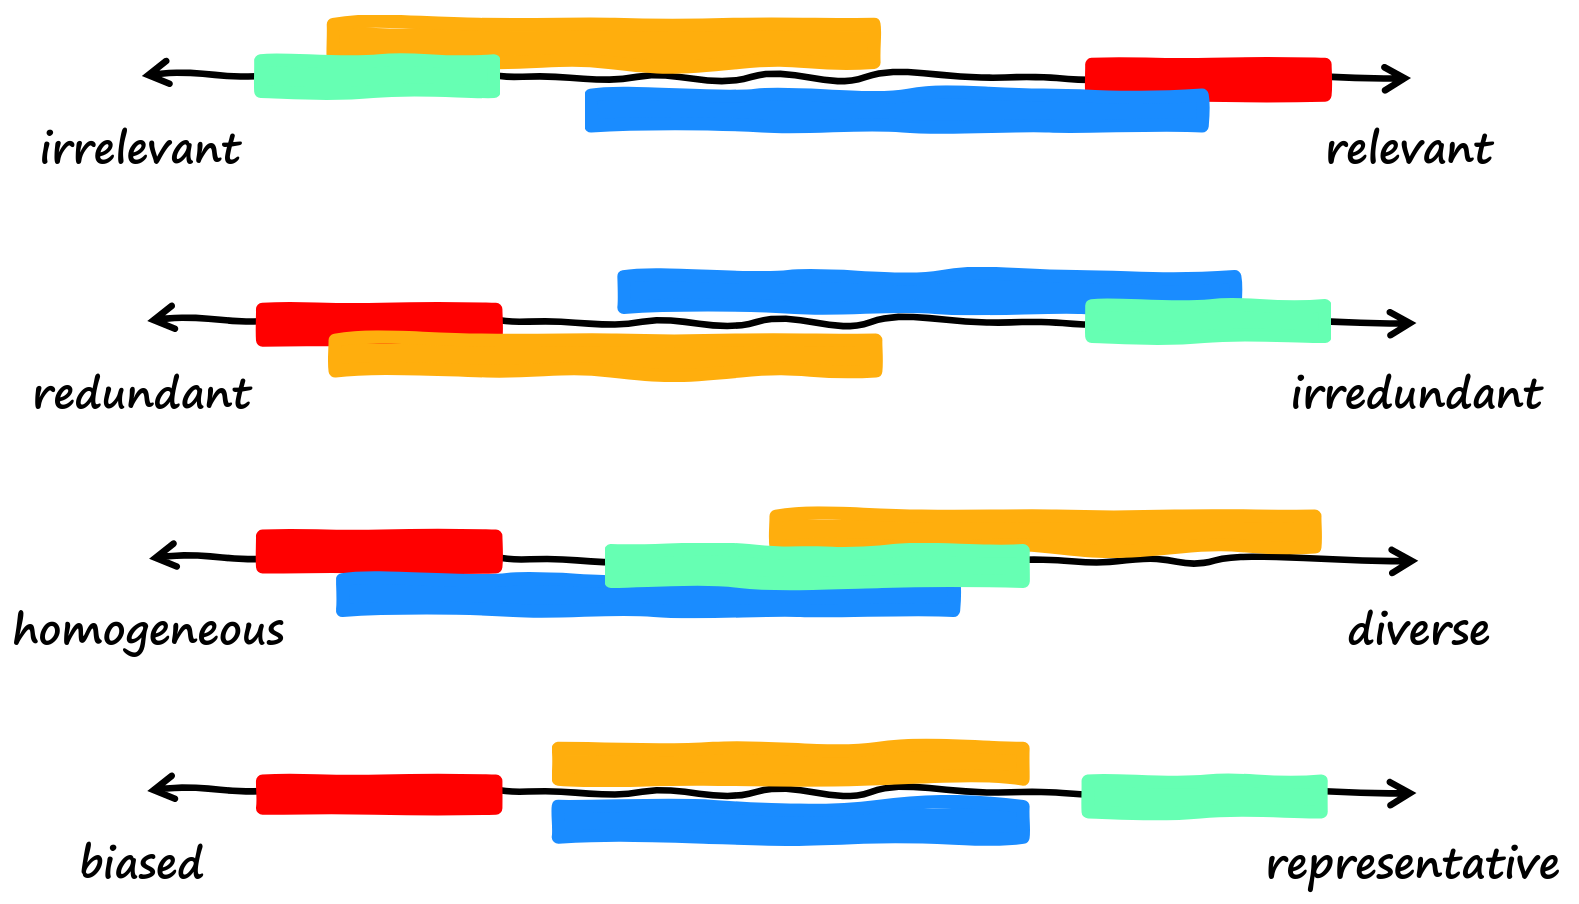
\includegraphics[width=\textwidth]{03_ranking/method_objectives.png}
	\caption[Different methods for semantic ranking achieve different trade-offs between our defined objectives.]{
		The discussed methods for semantic ranking achieve different trade-offs between our defined objectives.
	}
	\label{fig:suggestions/ranking/method_objectives}
\end{figure}

\noindent
To meet these requirements, we present four ranking methods and discuss how they balance all objectives differently~(\cref{fig:suggestions/ranking/method_objectives}): \emph{top-k selection}, \emph{probabilistic sampling}, \emph{clustering}, and \emph{probabilistic sampling from clusters}.

\paragraph{Top-k selection}
We sort all suggestions based on their relevance score and select the $k$ most relevant artifacts.

This approach maximizes the relevance of the ranking.
However, it can also maximize the redundancy of results if the relevance score depends on the similarity of artifacts because of the transitivity of similarity.
At the same time, diversity and representativeness are typically minimized because the selection explicitly focuses on most similar artifacts.

\paragraph{Probabilistic sampling}
We convert the relevance scores of the corpus into a probability distribution by scaling each relevance score exponentially to a probability $p_i$:
\begin{align}
	p_i = \frac{\exp \frac{R_i}{T}}{\sum_j \exp \frac{R_j}{T}}
\end{align}
Based on this probability distribution, we randomly sample $k$ unique artifacts.
Through a temperature parameter $T$, the probability distribution can be sharpened or flattened, modeling the ranking closer to top-k selection or uniform random selection, respectively.
This approach corresponds to the \emph{softmax} function used in several machine learning application.

In comparison with all other discussed methods, probabilistic sampling maximizes the diversity of the ranking if a medium to high temperature is used.
Similarly, the irredundancy of results is improved slightly.
However, results are significantly less relevant to the query or representative of the corpus.

\paragraph{Clustering}
We cluster the corpus into $k$ groups by using an algorithm such as k-means.
From each cluster, we select the most representative artifact (i.e., the center of the cluster).

Cluster-based selection maximizes the irredundancy and representativeness of the ranking.
On the downside, it does not honor the relevance of artifacts by any means.
Also, cluster centers present a lower diversity than sampling-based methods as they neglect outliers.

\paragraph{Probabilistic sampling from clusters}
We group the corpus into $k$ clusters, assign a probability to each cluster based on the relevance score of their center, and sample random clusters.
For each occurence of a cluster, we select the next most relevant artifact from it.
Similar to plain probabilistic sampling, this method can be controlled through a temperature parameter.

Cluster-based probabilistic sampling provides a trade-off between the other discussed methods with respect to all considered objectives:
in our experiments, it yielded a moderate relevance of suggestions that is between that of top-k selection and plain probabilistic sampling, a moderate representativeness close to probabilistic sampling, and a sufficient irredundancy and diversity between probabilistic sampling and clustering.

\begin{genericbox}{Failed attempts}
	We also experimented with two other ranking methods that did not yield usable results for us:

	\subparagraph{Explicitly amplifying diversity}
	We computed the diversity of each artifact as their average distance to all other artifacts and added that to the artifact score.
	Despite experimenting with different weights and scalings, we were not able to create rankings that would combine relevance and diversity in a satisfying way.

	\subparagraph{Clustering from an RBF-transformed embedding space}
	We transformed the embedding space of the corpus using a radial basis function (RBF) centered around the reference artifact before clustering it.
	We could not confirm our hypothesis that this approach would balance relevance and representativeness.
	In our experiments, the complexity and sensitivity of parameters rendered this approach impractical.
\end{genericbox}

\ParSep

In our prototype, we found probabilistic sampling from clusters to balance the different objectives in the most satisfying way and to be versatile for most applications.
For some use cases where no reference artifact has been specified, we use the plain clustering method instead.
